\documentclass[a4paper,12pt]{article}
\usepackage{blindtext}
\usepackage[utf8]{inputenc}
\usepackage{graphicx}
\usepackage{enumitem}
\usepackage{pgfplotstable}
\usepackage{booktabs}

\begin{document}
\begin{titlepage}
\center

\textsc{\LARGE Architectural Requirements}\\[1.5cm]
\textsc{\Large Project: Traffic Camera Image Analysis}\\[1.5cm]
\textsc{\large Client: DPSS, CSIR}\\[0.5cm]
\textsc{\large Team: Quadcore Productions}\\[0.5cm]

\begin{minipage}{0.4\textwidth}
\begin{flushleft} \large
\emph{Author(s):}\\
Mpho \textsc{Baloyi}\\
Hlengekile \textsc{Jita}\\
Mayimela \textsc{Moses}\\
Mbhele \textsc{Themba}\\
\end{flushleft}
\end{minipage}
~
\begin{minipage}{0.4\textwidth}
\begin{flushright} \large
\emph{Student number(s):} \\
14133670\\ % Student number
14077893\\
14019702\\
14007950\\
\end{flushright}
\end{minipage}\\

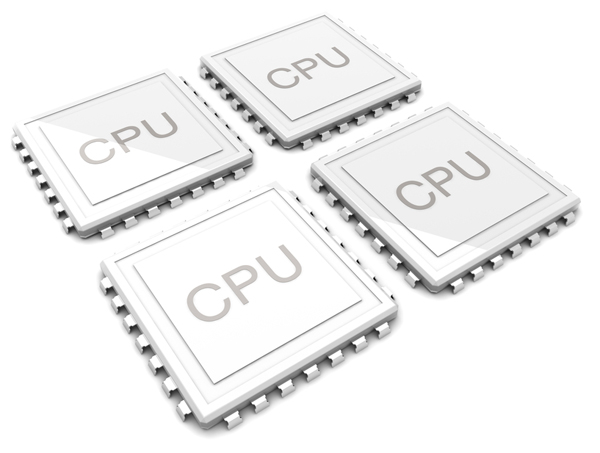
\includegraphics[width=\textwidth]{2012-quad-core-phones.jpg}

{\large University of Pretoria, Department of Computer Science}\\

{\large 29 July 2016}\\[3cm]

\vfil

\end{titlepage}

\newpage
\tableofcontents
\newpage

\newpage
\section{Versions}
\begin{table}[]
\begin{center}
    \caption{Document History}
    \pgfplotstabletypeset[
      multicolumn names, % allows to have multicolumn names
      col sep=comma, % the seperator in our .csv file
      display columns/0/.style={
		column name=$Value 1$, % name of first column
		column type={S},string type}, 
      display columns/1/.style={
		column name=$Value 2$,
		column type={S},string type},
	  display columns/2/.style={
		column name=$Value 3$,
		column type={S},string type},
	  display columns/3/.style={
		column name=$Value 2$,
		column type={S},string type},
	  every head row/.style={
		before row={\toprule},
		after row={\midrule}},
	  every last row/.style={after row=\bottomrule},
    ]{versionTable.csv} % filename/path to file
  \end{center}
\end{table}
\newpage

\section{Introduction}
This document describes the functional requirements and application design of the Traffic Camera Image Analysis System. The target system will run on a web server  and be accessed by users on an Android Application which will provide the users with the necessary functionality to access real-time traffic information that assists them with things such as avoiding traffic and choosing the best alternative routes. 

In this specification, we cover the use cases, their service contracts, required functionality and process specifications of the target system. The above, will be built on over time as the software is developed, as we are following an agile development methodology. In addition the domain model of the application as a whole will be provided.
\section{Vision}
For this project we aim to achieve a system that makes use of images obtained from highway cameras to provide users with up-to-date real-time traffic information. The system should simplify the user's travels by providing traffic information and notifying them before they depart of traffic conditions, calculating arrival times based on traffic conditions and help them select the most suitable route for their trips using the traffic information and additional metrics. Our vision for the target system is that it should be reliable and perform relatively quickly, both for user satisfaction and in order to be the an up-to-date traffic information system.
\section{Background}
As a commuter, traffic is something that is a part of everyday life, and it is not one of the more pleasurable aspects of life. Already there is software in place that assists us in dealing with this problem, such as Google Maps. This software uses the crowd-sourcing of GPS data in order to provide their up-to-date traffic information.

In our system,we want to take an image analysis approach to solve the same problem. We will make use of the publicly available SANRAL highway cameras to get images which can be found on https://www.i-traffic.co.za/traffic/cameras.aspx. Processing these images we will perform image analysis and determine the traffic conditions in the area of a camera. Using this information we will be able to generate information pertaining to user specified routes in order to provide the information necessary to help them avoid traffic and choose the most suitable routes in order to do so.
\section{System Scope}
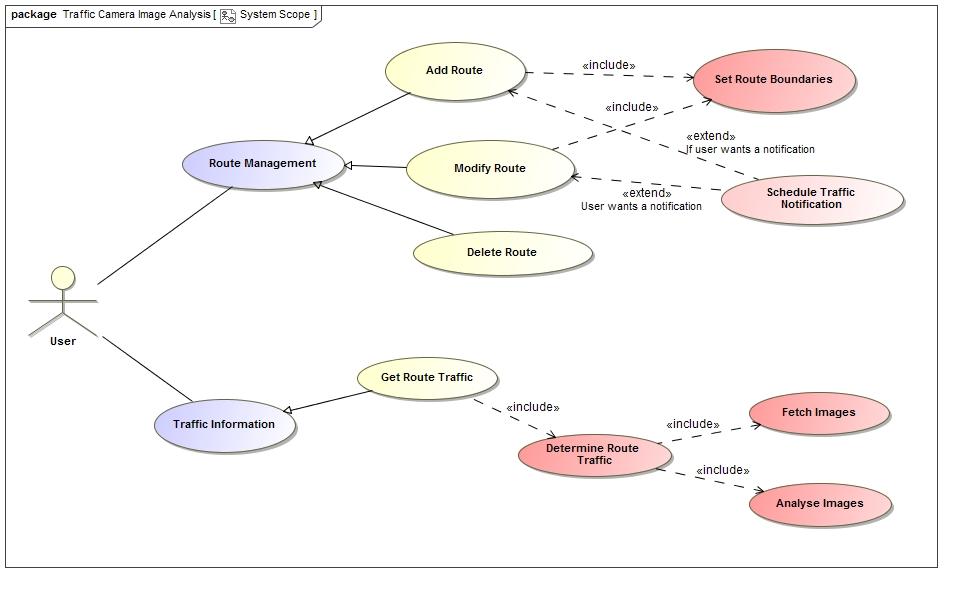
\includegraphics[width=\textwidth]{images/System_Scope.jpg}
\section{Functional Requirements}
\subsection{Use Cases}
The use cases for our system are described below. These use cases are the services that provide the user of the application some value. The following uses are listed in order of prioritization:
\begin{itemize}
\item Add Route 			(Critical)
\item Get Route Traffic		(Critical)
\item Modify Route			(Critical)
\item Delete Route			(Critical)
\item Schedule Notification (Important)
\item Route Optimization 	(Nice To Have)
\end{itemize}
\subsection{Service Contracts}
For each of the above services described above, there are are pre-conditions that must be met for the service to be carried out and post-conditions that are met to indicate the successful completion of a service. In addition the service contracts indicate what exceptions will be thrown in case the service fails.

\subsubsection{Add Route}
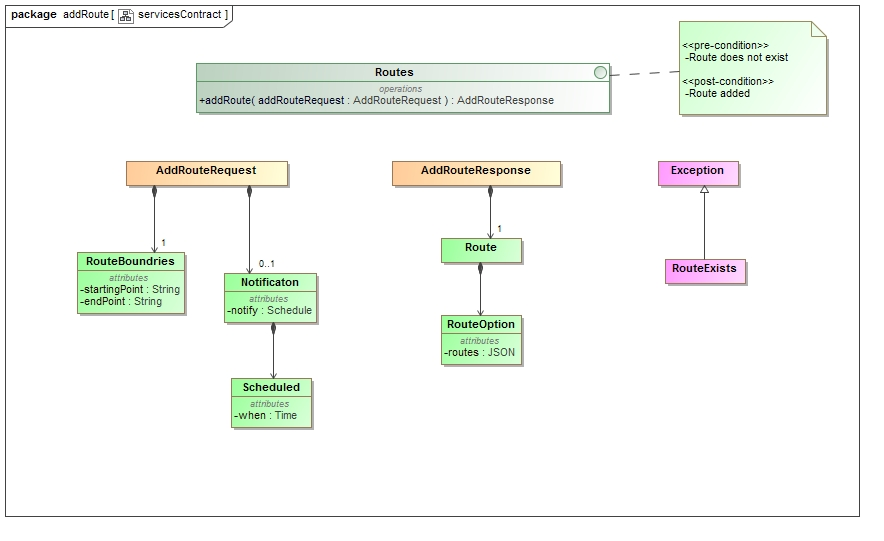
\includegraphics[width=\textwidth]{images/scAdd_Route.jpg}
\subsubsection{Modify Route} 
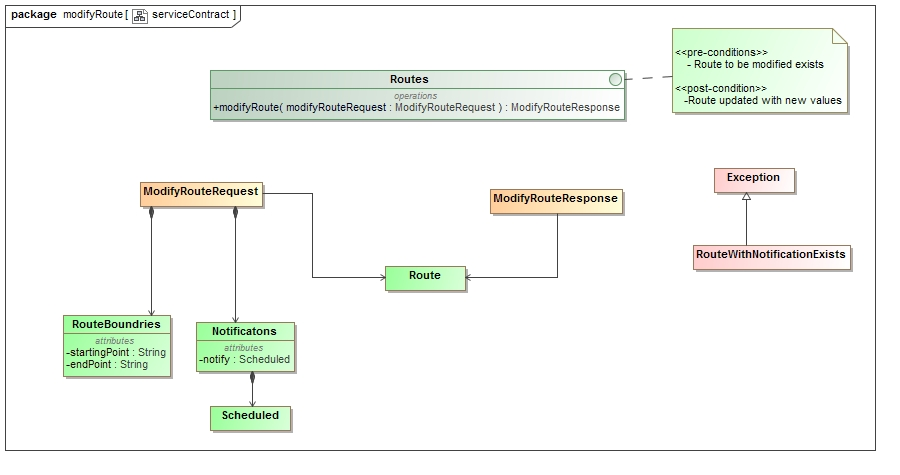
\includegraphics[width=\textwidth]{images/scModify_Route.jpg}
\subsubsection{Delete Route}
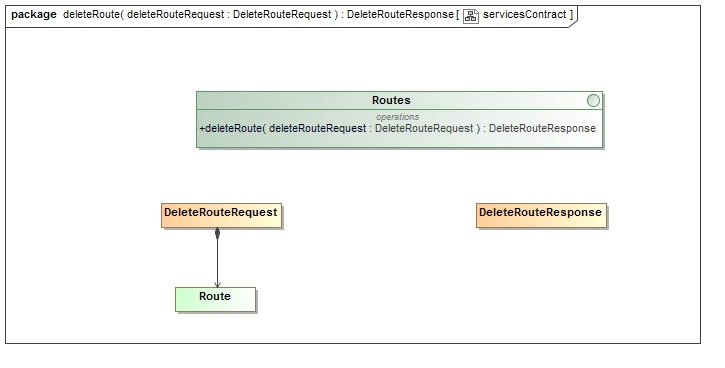
\includegraphics[width=\textwidth]{images/scDelete_Route.jpg}
\subsubsection{Get Route Traffic}
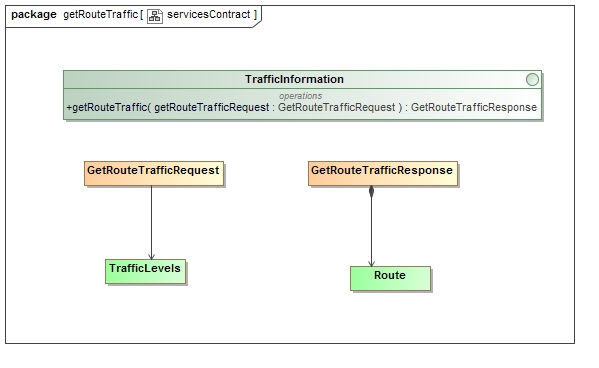
\includegraphics[width=\textwidth]{images/scDetermine_Traffic.jpg}
\subsubsection{Send Notification}
\includegraphics[width=\textwidth]{images/scSend_Notification.jpg}

\subsection{Required Functionality}
The use cases make use of other lower level functions in order to achieve their purpose. In the below diagrams for each high level use case, the lower level use cases that are required are described.
 
\subsubsection{Add Route}
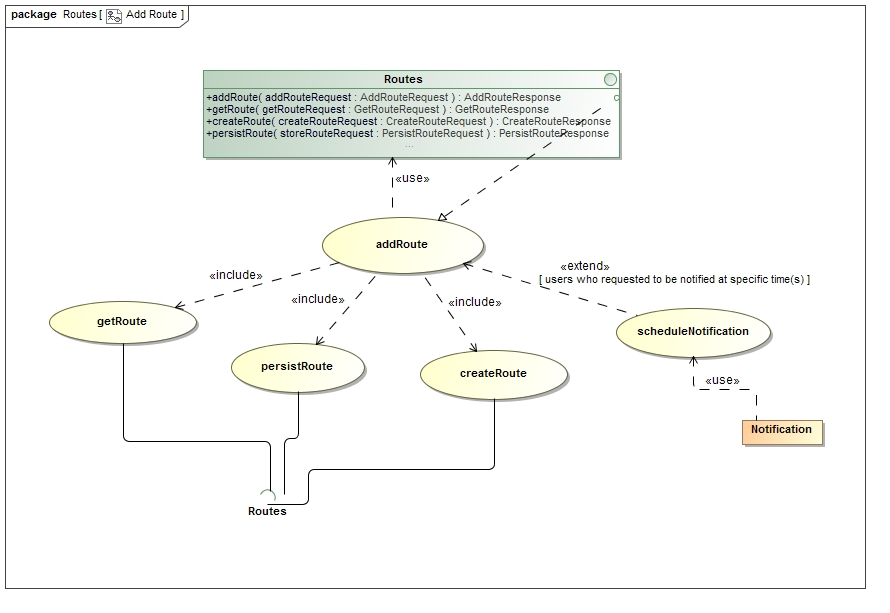
\includegraphics[width=\textwidth]{images/Add_Route.jpg}
\subsubsection{Modify Route} 
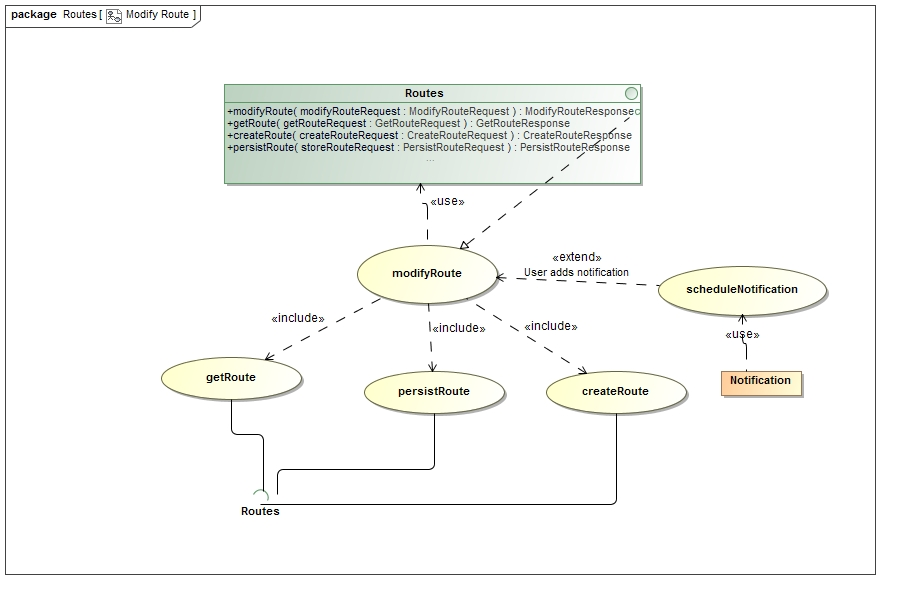
\includegraphics[width=\textwidth]{images/Modify_Route.jpg}
\subsubsection{Delete Route}
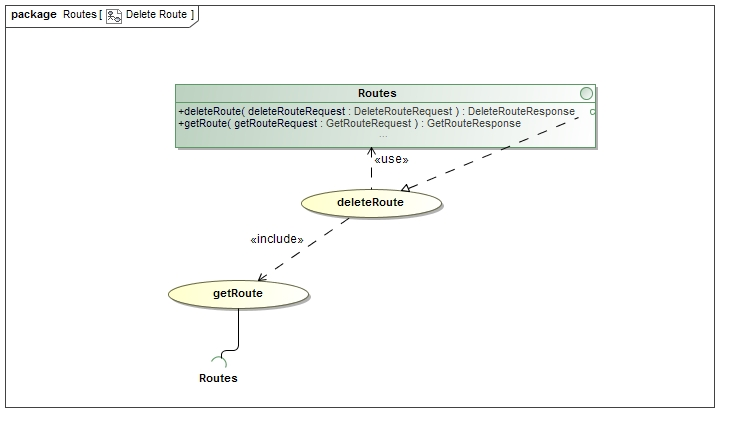
\includegraphics[width=\textwidth]{images/Delete_Route.jpg}
\subsubsection{Get Route Traffic}
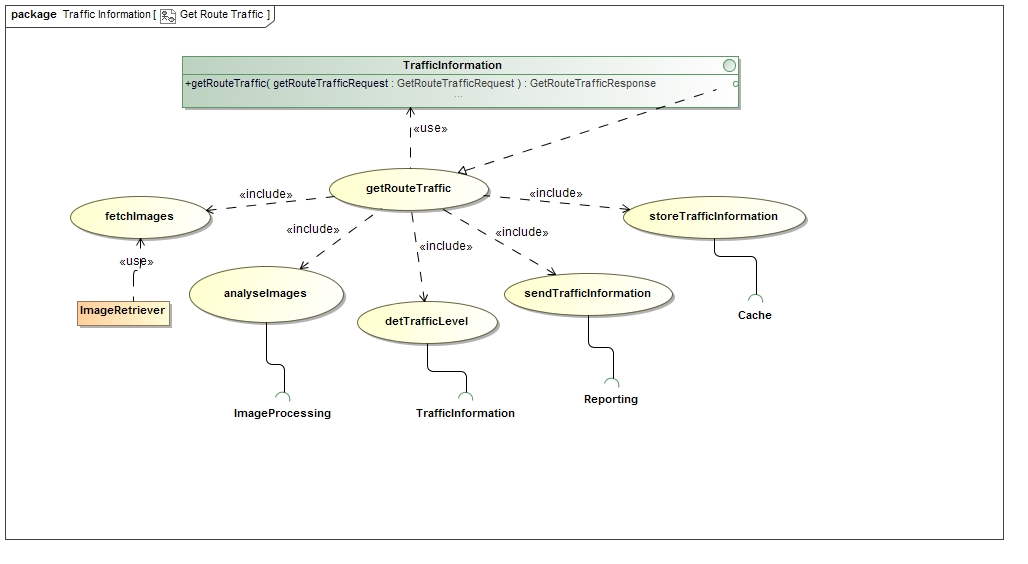
\includegraphics[width=\textwidth]{images/Get_Route_Traffic.jpg}

\subsection{Process Specification}
This section
\subsubsection{Add Route}
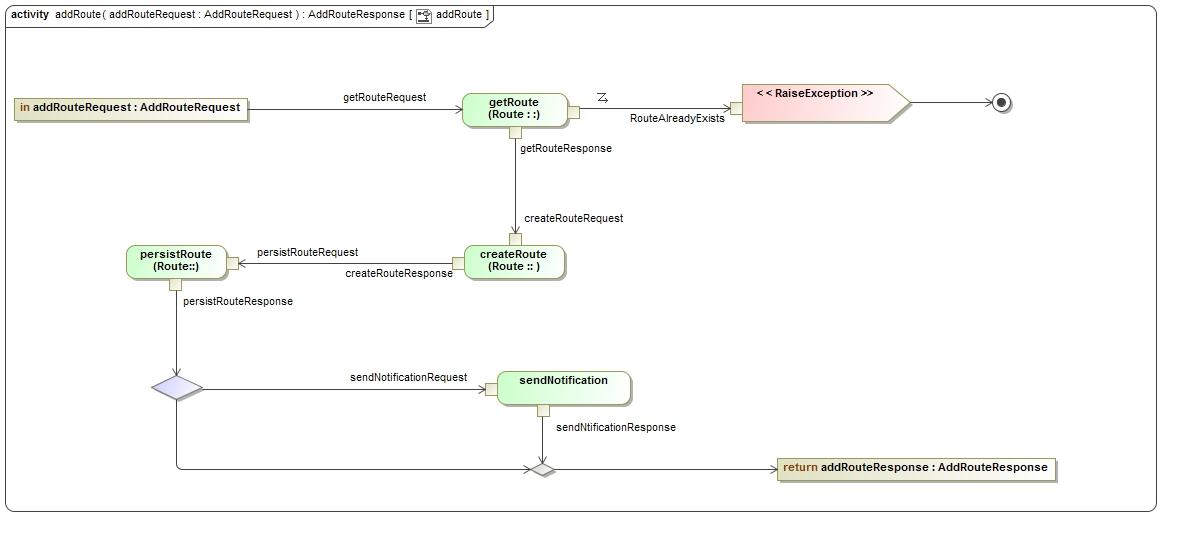
\includegraphics[width=\textwidth]{images/psAdd_Route.jpg}
\subsubsection{Modify Route}
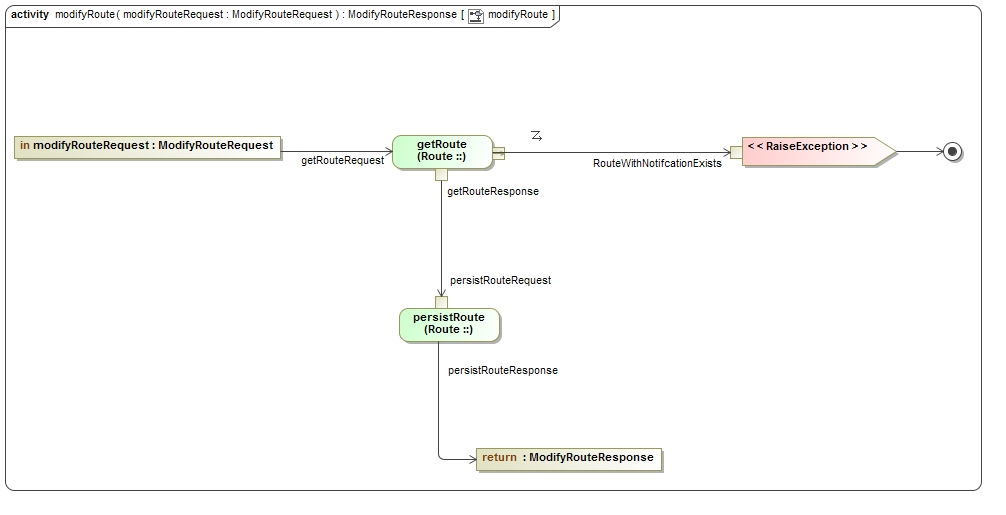
\includegraphics[width=\textwidth]{images/psModify_Route.jpg} 
\subsubsection{Get Route Traffic}
\includegraphics[width=\textwidth]{images/psGet_Route_Traffic.jpg}

\section{Domain Model}
\includegraphics[width=\textwidth]{images/Domain_Model.jpg}
\section{Open Issues}

\end{document}